\documentclass[11pt]{article}
% Use [review] for an anonymous submission with line numbers.
\usepackage[final]{acl}
\usepackage{times}
\usepackage{latexsym}
\usepackage{microtype}

\usepackage{amsmath,amssymb,amsfonts}
\usepackage{algorithmic}
\usepackage{graphicx}
\usepackage{textcomp}
\usepackage{xcolor}
\usepackage[utf8]{vietnam}
\usepackage[vietnamese, english]{babel}
\usepackage{booktabs}
\usepackage{tabularx}
\usepackage{array}
\usepackage{multirow}
\usepackage{url}
\def\BibTeX{{\rm B\kern-.05em{\sc i\kern-.025em b}\kern-.08em
    T\kern-.1667em\lower.7ex\hbox{E}\kern-.125emX}}

\newcommand{\envi}{EN$\rightarrow$VI}
\newcommand{\vien}{VI$\rightarrow$EN}

\begin{document}

\title{Document-Level English--Vietnamese Legal Machine Translation with a Fine-Tuned Small Language Model and a Structure-Aware Pipeline}

\author{Trần Đức Lâm, Lê Vân Anh, Phạm Thị Khánh Linh, Nguyễn Thị Hiền Trang \\
University of Engineering and Technology, \\
Vietnam National University, Hanoi, Vietnam}
% Add the authors' email addresses when available.

\maketitle

\begin{abstract}
We present our system for the VLSP 2026 shared task on document-level English--Vietnamese legal machine translation. Translating legal documents requires correct and consistent terminology, preserved structure and no omitted content, while the documents are often much longer than the amount of text a small model can read at once. To address this, we combine two components: LoRA fine-tuning of a translation model with fewer than 3 billion parameters on a cleaned and extended legal corpus, and a structure-aware Markdown pipeline that translates a document block by block, validates each output and re-translates the blocks that fail. On the public test set, the system reaches 70.87 BLEU for English-to-Vietnamese and 47.44 BLEU for Vietnamese-to-English. Controlled experiments show that fine-tuning on the processed data contributes the most, while the pipeline further improves quality in both directions at a cost of about two hours and 5~GB of GPU memory per direction.
\end{abstract}

\section{Introduction}
Legal documents pose a significant challenge to machine translation (MT) systems. They contain many specialised terms whose meanings differ markedly from general language, and they demand strict consistency across the whole document. A translation must also preserve every right, obligation, condition and exception of the source: a single omitted clause or a wrong number can change the legal effect completely. Finally, laws and decrees are long and hierarchically structured, with articles, clauses, points, tables and nested signature blocks, so they easily exceed the context window of small language models.

The VLSP 2026 shared task on document-level legal MT between English and Vietnamese adds practical constraints to these difficulties~\cite{vlsp2026}. A participating model must have fewer than 3 billion parameters, must run fully locally without calling any external API, and is evaluated not only on translation quality and terminology accuracy but also on inference time and peak memory. A system therefore has to be accurate, small and cheap at the same time.

To meet these requirements, we build our system on a translation model with 1.8 billion parameters and treat the task as document-level translation rather than translating each sentence independently. Our pipeline parses the Markdown structure of a document, translates runs of adjacent nodes instead of feeding the whole document to the model, checks every output against the source, and re-translates only the blocks that fail the checks. The model is fine-tuned with LoRA~\cite{hu2022lora} on a cleaned and extended legal corpus.

Our contributions are as follows.
\begin{itemize}
\item \textbf{A structure-aware document-level translation pipeline.} The pipeline parses a document into typed nodes, groups adjacent nodes into blocks without inserting markers into the text, checks each block with deterministic tests, re-translates failed blocks, batches blocks of similar length together, and stops generation early when the model starts repeating a phrase it has already produced (Section~\ref{sec:pipeline}).
\item \textbf{A cleaned and extended training corpus.} The corpus is built from the task data through alignment review, Unicode and tone-mark normalisation, a verified glossary, and additional paragraph-level and term-level pairs (Section~\ref{sec:data}).
\end{itemize}

Controlled experiments on two models in Section~\ref{sec:experiments} lead to three main findings. First, fine-tuning on the processed corpus is the largest single contributor to translation quality. Second, the pipeline further improves both the base model and the fine-tuned model, and grouping nodes without markers works better than translating each node separately. Third, the system reaches 70.87 BLEU for \envi{} and 47.44 BLEU for \vien{} on the public test set, using about two hours and 5~GB of GPU memory per direction on a single T4 GPU.

\section{Related Work}
\textbf{Small LLM-based translation models.} Recent open translation models are decoder-only LLMs adapted for MT: ALMA uses two-stage fine-tuning~\cite{xu2024alma}, Tower continues pre-training and then applies instruction tuning~\cite{alves2024tower}, NiuTrans.LMT focuses on Chinese and English~\cite{luo2025lmt}, and the Hunyuan family~\cite{zheng2025hunyuanmt}. We use Hy-MT2, whose 1.8B version supports 33 languages and, according to its authors, outperforms popular commercial APIs overall~\cite{zheng2026hymt2}. Encoder--decoder systems such as NLLB~\cite{nllb2022} cover many languages but do not follow instructions, so they cannot use terminology hints given in the prompt.

\textbf{English--Vietnamese translation.} The large public English--Vietnamese resources are sentence-level parallel corpora: PhoMT contains about 3 million sentence pairs~\cite{doan2021phomt}, and MTet contains 4.2 million training pairs with a multi-domain test set and the EnViT5 models~\cite{ngo2022mtet}. They do not provide structured legal documents, so we build paragraph-level and article-level training data as described in Section~\ref{sec:data}.

\textbf{Document-level and legal translation.} Context-aware neural MT shows that sentence-level systems lack consistency in deixis, ellipsis and lexical cohesion~\cite{voita2019context}; a survey of these model families is given by Maruf et al.~\cite{maruf2021survey}, and LLMs have been studied as document-level translators~\cite{wang2023docllm}. Recent legal translation work adapts pre-trained models to legal text, for example QLoRA fine-tuning of IndicTrans2 on the JUST-NLP 2025 legal corpus~\cite{singh2025indictrans2} and domain-specific fine-tuning of an open-weight LLM on EU legislation~\cite{lorini2026eu}. Our problem differs in that the unit is a whole Markdown document whose headings, article numbers and list labels must be preserved, so structure preservation and error recovery are part of the translation system rather than a post-check. We also guard against degenerate repetition, a known failure of probabilistic decoding~\cite{holtzman2020degeneration}, and apply a repetition penalty~\cite{keskar2019ctrl} only in the re-translation path.

\section{Method}
Our approach has three consecutive steps. First, we process the training data of the task to obtain a clean corpus suited to the legal domain (Section~\ref{sec:data}). Second, we fine-tune the translation model on this corpus (Section~\ref{sec:finetune}). Finally, the fine-tuned model runs inside a document-level pipeline in which a document is split into blocks, and each block is checked and re-translated if it fails (Section~\ref{sec:pipeline}).

\subsection{Training Data Processing}\label{sec:data}
\begin{figure*}[t]
\centering
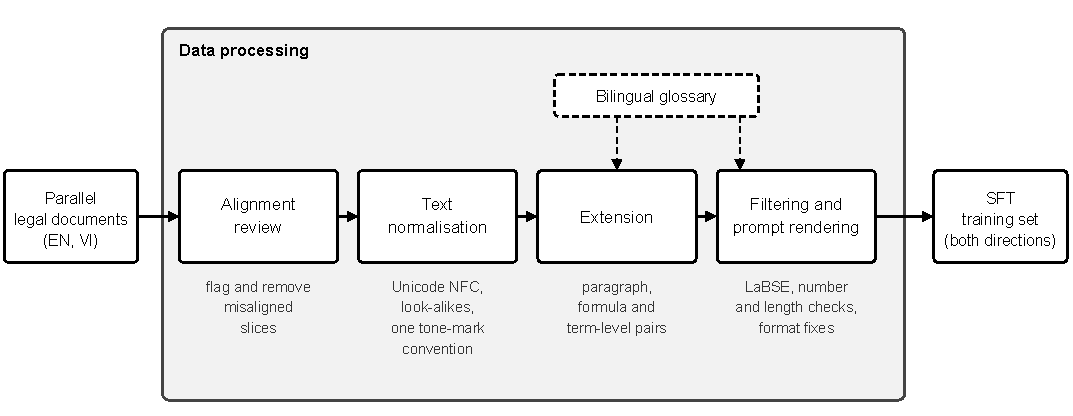
\includegraphics[width=\textwidth]{fig1.pdf}
\caption{Training-data processing, from the parallel data of the task to the supervised fine-tuning (SFT) set.}
\label{fig:data}
\end{figure*}

The training data of the task is parallel: it consists of pairs of legal documents, each with an English version and a Vietnamese version that correspond to each other. Each document is cut into several slices (views) at different levels: the preamble, a single article, a single clause, a group of adjacent articles, or the whole document. Slices are cut at the structural boundaries of legal texts (article, clause and article group), not at sentence boundaries. This keeps every sentence and every condition intact and exposes the model to inputs of different lengths, matching the blocks that the pipeline feeds to the model at inference time. A slice together with its translation forms one training row. We process the data in four steps (Fig.~\ref{fig:data}). Every removal or edit is stored in a separate decision file instead of modifying the source data, so every change can be traced and re-run. Table~\ref{tab:scale} compares the scale of the data before and after processing.

\begin{table}[t]
\centering
\begin{tabular}{lrr}
\toprule
Statistic & Initial & Final \\
\midrule
Training documents & 575 & 612 \\
Training rows & 54,134 & 82,203 \\
\bottomrule
\end{tabular}
\caption{Scale of the training data. ``Initial'' is the data after parsing. A row is one slice of a document with its translation, not a single sentence.}
\label{tab:scale}
\end{table}

\textbf{Alignment review.} The English and Vietnamese versions of a document sometimes do not match, for example when a clause is missing on one side or the decree numbers differ between the two languages. We flag 237 slices whose document codes or large numbers do not correspond between English and Vietnamese, review them, and remove 158 of them. Because an automatic flag is not proof of an error (a number may, for instance, be written in words on one side), these decisions are stored separately. When another slice of the same document contains the verbatim text of a removed segment, that slice is removed as well.

\textbf{Text normalisation.} Raw text mixes several encodings of the same character: decomposed Unicode, Cyrillic or other look-alike letters, invisible characters, legacy font fragments, and two conventions for placing the tone mark on the vowel groups \emph{oa}, \emph{oe} and \emph{uy}, such as \emph{h\`{o}a} and \emph{ho\`{a}}. A single normalisation function, which changed the tone mark of 41,431 words in the data, maps everything to Unicode NFC and to the tone-mark convention that is the majority in the training data. The same function is applied to the source text at inference so that the model sees the same character conventions in training and at test time.

\textbf{Glossary and data split.} A bilingual legal glossary of 442 pairs was checked against the training data and is used to build prompts that contain terminology hints during training; these make up about 24\% of the prompts. The data is split by document: all slices of the same document belong to exactly one of three sets, training, development (dev) and internal-test. This split avoids the content of one document appearing in both the training set and an evaluation set. In the final data the dev set is merged into the training set, so only the internal-test set of 23 documents is held out, and we use it to monitor the training loss.

\textbf{Extension and filtering.} The original rows are relatively long slices, from one clause to a group of several articles. To familiarise the model with shorter units as well, we add three groups of rows to the training set, listed in Table~\ref{tab:composition}. The first group is paragraph-level rows: individual paragraphs cut from the documents, much shorter than a complete article. The second group is hand-written formula phrases, including the national title, the motto, signer titles, document types, dates and document numbers. The third group is term rows, each a short pair of a term or an agency name that teaches the model how to translate it in context. In addition, we remove pairs that are still misaligned using the LaBSE similarity~\cite{feng2022labse} applied to the flagged pairs, extreme length ratios, mismatched national titles, and mismatched amounts or list labels. We manually correct typing errors and optical character recognition (OCR) errors that remain in the source data, and unify the thousands-separator format and the phrasing of fine amounts.

\begin{table}[t]
\centering
\small
\begin{tabular}{lr}
\toprule
Component & Rows \\
\midrule
Original rows after cleaning & 50,129 \\
Paragraph-level rows & 30,658 \\
Hand-written formula rows & 654 \\
Term rows from the training data & 690 \\
Term rows from public-test references & 72 \\
\midrule
\textbf{Total} & \textbf{82,203} \\
\bottomrule
\end{tabular}
\caption{Composition of the final training data.}
\label{tab:composition}
\end{table}

\subsection{Base Models and Fine-Tuning}\label{sec:finetune}
We experiment with two translation models with fewer than 3 billion parameters: Hy-MT2-1.8B, a dense model with 1.8 billion parameters~\cite{zheng2026hymt2}, and Index-Translate-2B, a publicly available translation model with 2 billion parameters~\cite{indexteam}. We fine-tune both on the same corpus with LoRA: the weights of the base model are frozen, and only the low-rank matrices added to the attention and MLP projections are trained.

\textbf{Loss function.} Each training sample consists of a prompt, which contains the translation instruction and the source text $x$, and a target translation $y=(y_1,\dots,y_T)$, where $y_T$ is the end-of-sequence token. The model is trained with supervised fine-tuning using the cross-entropy loss computed only on the tokens of the translation:
\begin{equation}
\mathcal{L}(\theta) = -\frac{1}{T}\sum_{t=1}^{T} \log p_\theta\big(y_t \mid x,\, y_{<t}\big).
\label{eq:loss}
\end{equation}
The tokens of the prompt are masked with the ignore index and do not contribute to the loss. We use no auxiliary loss and no label smoothing.

\textbf{Prompt.} Every pair uses a ``mixed'' prompt. With probability 0.5 we try to add terminology hints to the prompt: we look up the glossary pairs whose source term appears in the source text of the sample and whose translation also appears in the target translation of the sample. If any are found, the prompt lists up to 8 such pairs, preferring longer phrases. In all other cases, that is, when the 0.5 draw does not select hints or no pair is found, the prompt contains only the default instruction. At inference time the default instruction is always used. The prompts are given in Appendix~\ref{app:prompts}.

\subsection{Document-Level Translation Pipeline}\label{sec:pipeline}
The pipeline takes a Markdown document and returns the translation of the whole document in five steps, as shown in Fig.~\ref{fig:pipeline}: parse the document into nodes, group the nodes into blocks, translate each block, validate the outputs, re-translate failed blocks once, and finally select the best translation of each block and assemble the document. Each step is a separate module, so each can be changed and measured independently.

\begin{figure*}[t]
\centering
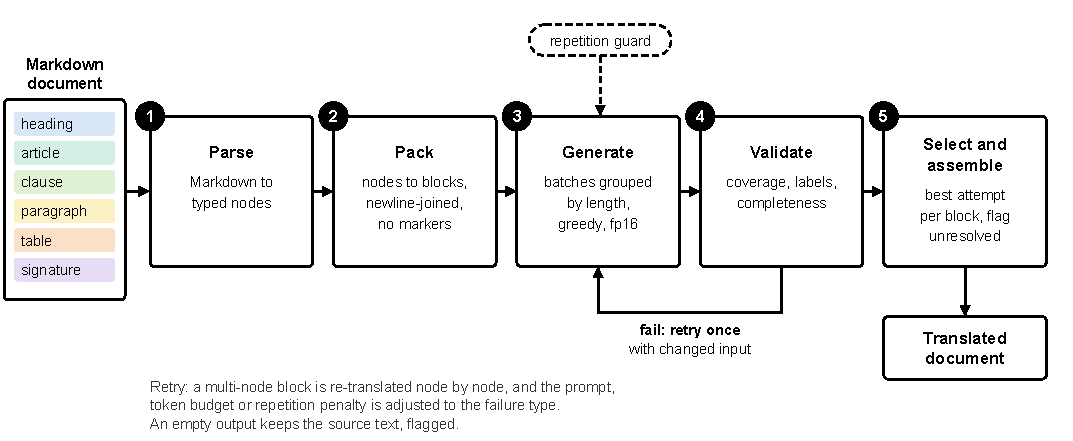
\includegraphics[width=\textwidth]{fig2.pdf}
\caption{Document-level translation pipeline. A Markdown document is parsed into nodes, grouped into blocks, translated in batches, validated, re-translated once if a block fails, and assembled into the translated document.}
\label{fig:pipeline}
\end{figure*}

\textbf{Parsing and grouping.} A rule-based parser, which does not use a model, converts the Markdown document into \emph{nodes}: headings, article and clause labels, paragraphs, table cells and signature blocks, such that concatenating the nodes reproduces the source text exactly. Adjacent prose nodes of the same scope, including headings, articles, clauses, points, list items and paragraphs, are merged into one \emph{block}. A block is closed when it reaches a limit on length or on the number of nodes and its last node ends with a full stop. A new article or a new chapter or section starts a new block; tables and signature blocks form blocks of their own. The nodes inside a block are joined only by newline characters, and no marker is inserted into the text. Each block is one translation unit, and the output of a block is not required to match the source line by line; instead, the system checks that each source paragraph has a corresponding translation exactly once.

\textbf{Validation and re-translation.} The output of each block is checked against three criteria. First, each source paragraph in the block must have a corresponding translation exactly once, without omission or duplication. Second, headings and numbered labels, such as article and clause names, must be preserved. Third, the translation must be complete, meaning that the model produces the end-of-sequence token before reaching the limit on the number of tokens it may generate, called the output budget, and that the translation does not loop. A block that fails any criterion is re-translated with a modified input chosen according to the type of failure. If a label was lost, we add an instruction to keep the source labels. If a block hit the budget, we re-translate it with a fallback budget. If the translation repeated itself, we apply a repetition penalty, a parameter that lowers the probability of selecting tokens that were just generated. A block with several nodes is split and each node is translated separately to avoid line misalignment. Each block is re-translated at most once to keep the running time within limits; that is, a block is translated at most twice: the first pass and at most one re-translation. The system keeps the better translation between the first pass and the re-translation. A block that still fails afterwards is called unresolved; its best translation is still written to the output and flagged with a warning. If the model returns an empty output for a paragraph, the system copies the untranslated source paragraph into the output and flags it as well. In this way, no source paragraph disappears from the translation without a signal to the user.

\textbf{Decoding, batching and repetition guard.} Decoding is the process in which the model generates the translation one token at a time. There are two main options: sampling, which draws a token at random from the probability distribution, and greedy decoding, which always picks the token with the highest probability. The pipeline uses greedy decoding in fp16 precision. The output budget depends on the translation direction and on the source length, because a Vietnamese text needs about 1.5 times as many tokens as the English text. To speed up inference, blocks are sorted by source length and split into batches of blocks with similar lengths, which reduces the number of padding tokens. The batch size is chosen by calibration on each GPU. Greedy decoding sometimes falls into degenerate repetition, in which the model repeats a phrase it has already generated and never stops. A detector running on the GPU periodically inspects the tokens just generated and stops generation early when it detects a loop. The stopped block is considered incomplete and enters the re-translation pass above, where the repetition penalty is applied; the first pass of every block does not use the penalty.

\section{Experiments}\label{sec:experiments}
\subsection{Experimental Setup}
\textbf{Data.} We report results on the public test set of 50 document pairs, each translated in both directions. During development we use a dev set split by document from the training data supplied by the organisers. The final training data contains 82,203 rows (Table~\ref{tab:scale}).

\textbf{Fine-tuning.} Both Hy-MT2-1.8B and Index-Translate-2B are fine-tuned with LoRA under supervision, using the cross-entropy loss in Eq.~\eqref{eq:loss}, on two T4 GPUs. For the weight matrix $W_0 \in \mathbb{R}^{d \times k}$ of a projection, LoRA learns two matrices $B \in \mathbb{R}^{d \times r}$ and $A \in \mathbb{R}^{r \times k}$ with $r \ll \min(d, k)$, and uses the weight
\begin{equation}
W = W_0 + \frac{\alpha}{r} B A,
\label{eq:lora}
\end{equation}
where $W_0$ is kept frozen. For Hy-MT2 we use $r = 64$, $\alpha = 128$ and dropout 0.05 on the query, key, value, output, gate, up and down projections. This configuration has 77.6 million trainable parameters, 4.15\% of the total number of parameters of the model with the adapter; the computation is given in Appendix~\ref{app:lora}. The model is trained in fp16 precision. The length of a training sample $(x,y)$ is counted with the tokenizer of the model after applying the chat template:
\begin{equation}
n(x, y) = n_{\mathrm{special}} + |P(x)| + |y|, \qquad n_{\mathrm{special}} = 5,
\label{eq:len}
\end{equation}
where $|P(x)|$ is the number of tokens of the prompt (the translation instruction, the source text and, if present, the terminology hints), $|y|$ is the number of tokens of the translation, and $n_{\mathrm{special}}$ counts the five special tokens of the template: the beginning-of-sequence token, the user tag, the assistant tag, the end-of-sequence token and the closing token of the template. A sample with $n(x,y)>3{,}072$ is dropped instead of being truncated, to prevent the model from learning truncated translations; in the final training run no training sample was dropped.

\textbf{Inference.} Inference uses the pipeline of Section~\ref{sec:pipeline} with greedy decoding in fp16, at most 768 source tokens or 8 nodes per block, batch size 8 and one re-translation pass. The repetition penalty is 1.0 in the first pass and 1.15 when a block is re-translated because of repetition. Each direction runs on its own T4 GPU on Kaggle with the Hugging Face Transformers library.

\textbf{Metrics.} We report corpus-level SacreBLEU~\cite{post2018sacrebleu} with the 13a tokenizer, SacreBLEU's default tokenizer, which splits text into tokens on whitespace and punctuation before counting $n$-grams, case-sensitive, together with chrF~\cite{popovic2015chrf}, computed on raw outputs and raw references without normalising either side. BLEU~\cite{papineni2002bleu} is computed at the corpus level:
\begin{equation}
\begin{aligned}
\mathrm{BLEU} &= \mathrm{BP}\cdot\exp\Big(\sum_{n=1}^{4}\tfrac{1}{4}\log p_n\Big),\\
\mathrm{BP} &= \min\big(1,\;e^{\,1-r/c}\big),
\end{aligned}
\label{eq:bleu}
\end{equation}
where $p_n$ is the modified $n$-gram precision computed over the whole corpus, $c$ is the length of the translation and $r$ is the length of the reference. chrF is the weighted harmonic mean of the character $n$-gram precision $\mathrm{chrP}$ and recall $\mathrm{chrR}$, up to order 6 and without word $n$-grams:
\begin{equation}
\mathrm{chrF}_\beta = (1+\beta^2)\,\frac{\mathrm{chrP}\cdot\mathrm{chrR}}{\beta^2\,\mathrm{chrP}+\mathrm{chrR}},\quad \beta = 2.
\label{eq:chrf}
\end{equation}
Confidence intervals are estimated with paired bootstrap resampling over documents~\cite{koehn2004significance}. In each resample $b = 1,\dots,B$ we draw 50 documents with replacement from the 50 documents of the test set, compute the corpus-level BLEU of the two systems on the same drawn set, and record the difference
\begin{equation}
\Delta_b = \mathrm{BLEU}_b(S_2) - \mathrm{BLEU}_b(S_1).
\label{eq:boot}
\end{equation}
The 95\% confidence interval is the range from the 2.5th to the 97.5th percentile of $\{\Delta_b\}$. We use $B = 2{,}000$ for the main comparisons and $B = 1{,}000$ for the node-grouping experiment.

\subsection{Results}
We compare three systems on both models, each adding one component to the previous one. System (1) is the base model translating paragraph by paragraph without the pipeline. System (2) is the base model run through the pipeline. System (3) is the fine-tuned model run through the pipeline, and it is our proposed system. Comparing (1) with (2) isolates the contribution of the pipeline, and comparing (2) with (3) isolates the contribution of fine-tuning.

\textbf{Pipeline and fine-tuning.} Table~\ref{tab:main} shows that the pipeline improves the translation quality of the base model in both directions, and the improvement is statistically significant, i.e., the 95\% confidence interval of the BLEU difference does not contain 0. Fine-tuning on the cleaned and extended corpus improves quality far more than the pipeline alone and is the largest contribution. The same trend appears for Index-Translate, which shows that the conclusion does not hold for a single model only. The \vien{} direction scores lower than \envi{} for every system. We believe the gap is partly due to the two directions using non-equivalent score scales: BLEU with the 13a tokenizer does not segment Vietnamese words, whereas the chrF difference between the two directions is only about 5 points. Another part is due to English translations that are phrased differently from the reference where the data sources do not agree on translation conventions.

\textbf{Model choice.} According to Table~\ref{tab:main}, before fine-tuning and without the pipeline, Index-Translate scores higher than Hy-MT2 in both directions. However, each model was run with the decoding recommended for it, namely sampling for Hy-MT2 and greedy decoding for Index, so this is not a controlled comparison. After fine-tuning, Hy-MT2 scores higher in both directions, so we choose Hy-MT2-1.8B as our main system. The analyses of node grouping and cost below use only this model.

\begin{table*}[t]
\centering
\begin{tabular}{llcccc}
\toprule
 & & \multicolumn{2}{c}{\envi{}} & \multicolumn{2}{c}{\vien{}} \\
\cmidrule(lr){3-4}\cmidrule(lr){5-6}
Model & System & BLEU & chrF & BLEU & chrF \\
\midrule
Hy-MT2-1.8B & (1) Base, no pipeline & $36.53 \pm 0.02$ & 64.78 & $28.87 \pm 0.04$ & 68.26 \\
 & (2) Base + pipeline & 39.96 & 65.43 & 30.27 & 68.89 \\
 & (3) Fine-tuned + pipeline & \textbf{70.87} & \textbf{84.48} & \textbf{47.44} & \textbf{79.50} \\
\midrule
Index-Translate-2B & (1) Base, no pipeline & 43.96 & 68.74 & 31.22 & 70.55 \\
 & (2) Base + pipeline & 45.49 & 69.26 & 32.38 & 71.15 \\
 & (3) Fine-tuned + pipeline & 62.59 & 78.89 & 41.76 & 76.48 \\
\bottomrule
\end{tabular}
\caption{Results on the public test set, 50 documents per direction. In row (1), Hy-MT2 translates paragraph by paragraph with sampling following its model card, and the value is the mean $\pm$ standard deviation over three seeds. Index uses greedy decoding, so the two (1) rows are not directly comparable.}
\label{tab:main}
\end{table*}

\textbf{Pipeline design.} In the first version of the pipeline, we compared three ways of grouping nodes (Table~\ref{tab:design}). Design C translates each node as a separate request, design A groups adjacent nodes with explicit markers, and design B groups adjacent nodes joined only by newline characters, without markers. Both A and B are better than C, with confidence intervals that do not contain 0 in both directions, because translating node by node loses the context of the neighbouring nodes. B scores no lower than A, and the difference is statistically significant only for \envi{}; B also avoids the loss of markers and shortens the running time. We therefore choose B and extend it to the legal prose blocks of Section~\ref{sec:pipeline}.

\begin{table}[t]
\centering
\footnotesize
\resizebox{\columnwidth}{!}{%
\begin{tabular}{lcccc}
\toprule
 & \multicolumn{2}{c}{\envi{}} & \multicolumn{2}{c}{\vien{}} \\
\cmidrule(lr){2-3}\cmidrule(lr){4-5}
Design & BLEU & chrF & BLEU & chrF \\
\midrule
A: grouped, with markers & 68.70 & 83.24 & 46.37 & 79.01 \\
B: grouped, no markers & \textbf{68.90} & \textbf{83.39} & \textbf{46.62} & \textbf{79.17} \\
C: one node per request & 67.69 & 82.64 & 45.23 & 78.23 \\
\bottomrule
\end{tabular}}
\caption{Three ways of grouping nodes on a model fine-tuned on about 53.5 thousand training rows, in the first version of the pipeline. Settings: repetition penalty 1.05, batch size 4, one run per design.}
\label{tab:design}
\end{table}

\subsection{Cost}
Since Hy-MT2-1.8B was chosen as the main model in the previous subsection, we analyse here the computational cost of systems (1), (2) and (3) based on Hy-MT2-1.8B, as reported in Table~\ref{tab:cost}. The system translates the whole public test set in about 2.0 hours for \envi{} and 1.4 hours for \vien{} on one T4 GPU per direction, with a peak GPU memory of about 5~GB, well within a 16~GB card. The first version of the pipeline needed 4.6 and 2.9 hours for the model fine-tuned on about 53.5 thousand rows, so the final runtime roughly halves the running time. Fine-tuning does not add cost: system (3) is even faster than system (2). For \envi{}, system (3) needs fewer re-translation requests, 836 against 962, and leaves fewer unresolved blocks, 26 against 110. For \vien{}, it needs more re-translation requests, 1,443 against 1,147, but still leaves fewer unresolved blocks, 208 against 241. System (1) is fast because it makes a single call per paragraph and does not validate or re-translate its output.

\begin{table}[t]
\centering
\footnotesize
\resizebox{\columnwidth}{!}{%
\begin{tabular}{lcccc}
\toprule
 & \multicolumn{2}{c}{Time (s)} & \multicolumn{2}{c}{Peak GPU (GB)} \\
\cmidrule(lr){2-3}\cmidrule(lr){4-5}
System & \envi{} & \vien{} & \envi{} & \vien{} \\
\midrule
(1) Base, per seed & $\sim$4.0k & $\sim$4.1k & 5.41 & 4.90 \\
(2) Base + pipeline & 8,111 & 5,326 & 5.34 & 5.15 \\
(3) Fine-tuned + pipeline & 7,229 & 4,871 & 4.96 & 5.25 \\
\bottomrule
\end{tabular}}
\caption{Running time and peak GPU memory on one T4 GPU per direction, with Hy-MT2-1.8B.}
\label{tab:cost}
\end{table}

\section{Limitations and Discussion}
Our system has several limitations. The configuration was chosen on the public test set, and 72 training rows come from the references of this set, so the reported scores may be somewhat optimistic for unseen documents. We evaluate only with the automatic metrics BLEU and chrF, so we have not directly checked whether a translation conveys the correct legal meaning, nor whether terms are translated consistently across a whole document. Some misaligned pairs remain undetected in the training data, and the \vien{} direction remains clearly lower than \envi{}.

These limitations point to several issues for further discussion. Regarding evaluation, terminology and legal accuracy should be assessed by humans or by an LLM to learn how far BLEU and chrF reflect the legal quality of a translation. Regarding data, a separate ablation of each cleaning step would show which step contributes most to the improvement from fine-tuning, and unifying the translation conventions across data sources may help the \vien{} direction. Regarding inference, terminology hints are currently used only in training; using them at inference time is a direction that has not yet been investigated systematically.

\section{Conclusion}
We presented a document-level legal MT system for English--Vietnamese that consists of a model with 1.8 billion parameters, fine-tuned on a cleaned and extended legal corpus, and a structure-aware document pipeline. Controlled experiments on two models show three results. First, fine-tuning on the processed corpus is the largest contributor to translation quality. Second, the pipeline further improves the quality of both the base model and the fine-tuned model, where grouping nodes without markers is better than translating each node separately, and the validation-and-re-translation mechanism repairs failed blocks. Third, the system reaches 70.87 BLEU for \envi{} and 47.44 BLEU for \vien{} on the public test set, using about two hours and 5~GB of GPU memory per direction on a single T4 GPU.

\bibliography{references}

\clearpage
\appendix

\section{Prompts}\label{app:prompts}
The prompts below are sent as the user turn of the chat template of each model. In the prompts, \texttt{\{src\}} is the text of the unit and \texttt{\{tgt\}} is ``English'' or ``Vietnamese''.

\textbf{Hy-MT2-1.8B.}
\begin{itemize}\raggedright
\item Default: \texttt{Translate the following text into \{tgt\}. Note that you should only output the translated result without any additional explanation:} followed by a blank line and \texttt{\{src\}}.
\item With terminology, used only in training: \texttt{Reference the following translations:} followed by the list \texttt{\{refs\}}, a blank line, then \texttt{Translate the following text into \{tgt\}. Note that you must ONLY output the translated result without any additional explanation:}, a blank line and \texttt{\{src\}}. Each line of \texttt{\{refs\}} has the form ``source term translates to target term'', with at most 8 pairs.
\end{itemize}

\textbf{Index-Translate-2B.} The standard translation prompt of the model, which is a Chinese instruction that asks the model to translate the given text from the source language into the target language and to output the translation directly without any explanation. The names of the source and target languages are written in Chinese, and the thinking mode is turned off.

\section{Hyperparameters}\label{app:hyper}
Hy-MT2-1.8B is fine-tuned in two consecutive passes: the first trains an adapter from the base model on about 53.5 thousand rows, and the second continues from that adapter on all 82,203 rows with a lower learning rate.

\begin{table*}[t]
\centering
\footnotesize
\begin{tabular}{p{0.28\textwidth}p{0.62\textwidth}}
\toprule
Item & Value \\
\midrule
Base model (Hy-MT2) & Hy-MT2-1.8B, fixed revision \texttt{9a341cd1b679d3efd23b\allowbreak 46e847b01745a71ed792} \\
Base model (Index) & \texttt{IndexTeam/Index-Translate-2B}, revision \texttt{a516854233b170140b57\allowbreak d36b48d7148c0edebabb} \\
LoRA (Hy-MT2) & $r=64$, $\alpha=128$, dropout 0.05; q, k, v, o, gate, up, down; 77.6 million parameters (4.15\%) \\
Data (Hy-MT2) & Pass one: about 53.5 thousand rows; pass two: 82,203 rows \\
Learning rate (Hy-MT2) & Pass one: $2\times10^{-4}$; pass two: $5\times10^{-5}$ (cosine decay to 10\%, 25 warm-up steps) \\
Epochs, steps & 1 epoch per pass; pass two: 2,569 steps \\
Effective batch size & $1 \times 16$ accumulation steps $\times$ 2 GPUs $= 32$ \\
Precision, maximum length & fp16 DDP, 3,072 tokens \\
Weight decay, gradient clipping & 0.0, 1.0 \\
Seed, hardware & 42, Kaggle 2$\times$T4 \\
Index-Translate-2B & \emph{to be completed} \\
Decoding (submission) & greedy, fp16, repetition penalty 1.0 in the first pass; 1.15 when re-translating after a loop \\
Re-translation & one pass \\
Repetition detection & every 32 generated steps, on the GPU \\
Source block & closed after exceeding 768 tokens or 8 nodes, at a node that ends with a full stop \\
Output budget & \envi{}: $2.5 s + 128$; \vien{}: $1.25 s + 128$; at least 256 \\
Inference batch size & 8 (calibrated between 8 and 16) \\
Context limit & 8,192 tokens \\
Post-processing & none \\
\bottomrule
\end{tabular}
\caption{Hyperparameters.}
\label{tab:hyper}
\end{table*}

The SHA-256 of the second-pass adapter (Hy-MT2) is {\footnotesize\texttt{30b5fc68a31c3de3d722\allowbreak a6dee5484aaf98c4f6b9d7\allowbreak b41fb55ac70f6d23a3ba89}}.

\section{Computing the Number of LoRA Parameters}\label{app:lora}
For a projection $m$ with weight matrix of size $d_{\mathrm{out}}^{(m)} \times d_{\mathrm{in}}^{(m)}$, LoRA adds the two matrices $B$ and $A$, that is, $r\,\big(d_{\mathrm{in}}^{(m)} + d_{\mathrm{out}}^{(m)}\big)$ parameters. Let $\mathcal{M}$ be the set of projections that receive LoRA in one layer and $L$ the number of layers; the total number of trainable parameters is
\begin{equation}
N_{\mathrm{LoRA}} = L \sum_{m \in \mathcal{M}} r\,\big(d_{\mathrm{in}}^{(m)} + d_{\mathrm{out}}^{(m)}\big),
\end{equation}
and the ratio to the total number of parameters of the model with the adapter is
\begin{equation}
\rho = \frac{N_{\mathrm{LoRA}}}{N_{\mathrm{base}} + N_{\mathrm{LoRA}}}.
\end{equation}
With $L=32$, $r=64$ and the sizes of the seven projections in Table~\ref{tab:loraparams}, $N_{\mathrm{LoRA}} = 77{,}594{,}624$ and $\rho = 77{,}594{,}624 / (1{,}791{,}080{,}448 + 77{,}594{,}624) \approx 4.15\%$.

\begin{table}[t]
\centering
\footnotesize
\begin{tabular}{lrrr}
\toprule
Projection & $d_{\mathrm{in}}$ & $d_{\mathrm{out}}$ & Params per layer \\
\midrule
query & 2,048 & 2,048 & 262,144 \\
key & 2,048 & 512 & 163,840 \\
value & 2,048 & 512 & 163,840 \\
output & 2,048 & 2,048 & 262,144 \\
gate & 2,048 & 6,144 & 524,288 \\
up & 2,048 & 6,144 & 524,288 \\
down & 6,144 & 2,048 & 524,288 \\
\midrule
\textbf{Total per layer} & & & \textbf{2,424,832} \\
\textbf{Total, 32 layers} & & & \textbf{77,594,624} \\
\bottomrule
\end{tabular}
\caption{LoRA parameters per projection (Hy-MT2-1.8B, $r=64$). Each projection contributes $r\,(d_{\mathrm{in}}+d_{\mathrm{out}})$ parameters per layer; the model has 32 layers.}
\label{tab:loraparams}
\end{table}



\end{document}
